\section{Strumenti utilizzati}

Per la realizzazione della tesi sono state usati i seguenti strumenti:
\paragraph{•} Arduino 
\paragraph{•} NFC Shield v2.0
\paragraph{•} NFC Tag
\paragraph{•} Java
\paragraph{•} NoSQL Database

\subsection{Arduino Uno}
Arduino è una piattaforma hardware composta da una serie di schede elettroniche dotate di un microcontrollore. È stata ideata e sviluppata nel 2003 da alcuni membri dell'Interaction Design Institute di Ivrea come strumento per la prototipazione rapida e l'utilizzo in vari ambiti, per esempio la robotica e la domotica.
\begin{center}
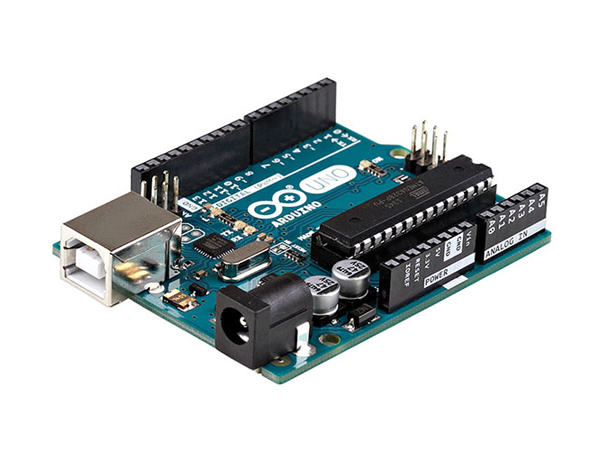
\includegraphics[scale=0.5]{arduino}
\end{center}
\subsection{NFC Shield v2.0}
Le shield sono schede che possono vengono inserite sopra l'Arduino, permettono l'estensione delle capacità della scheda stessa.La shield usata un questo progetto è quella NFC composta da un'antenna che collegandosi ad Arduino abilita la capacità di leggere/scrivere sui chip NFC
\begin{center}
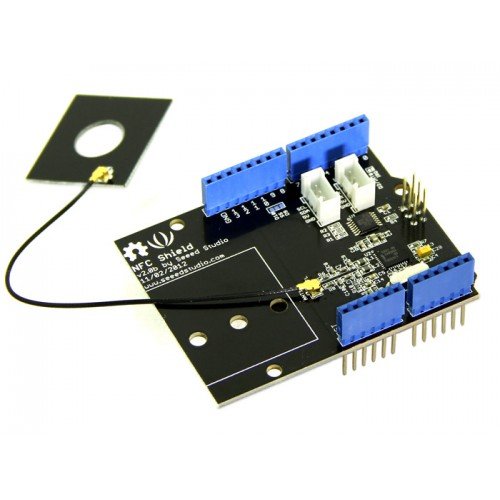
\includegraphics[scale=0.5]{shield}
\end{center}
\subsection{NFC Tag}
La tecnologia NFC  è una combinazione d'identificazione senza contatto (\textbf{RFID}) e altre tecnologie di connettività.NFC permette una comunicazione bidirezionale: quando due apparecchi NFC (initiator e target) vengono accostati entro un raggio di 4 cm, viene creata una rete peer-to-peer tra i due ed entrambi possono inviare e ricevere informazioni.
\\La tecnologia NFC opera alla frequenza di 13,56 MHz e può raggiungere una velocità di trasmissione massima di 424 kbit/s.
\\Il formato dei chip NFC usato nel progetto è \textbf{NDEF} [SPIEGAZIONE NDEF ?]
\subsection{Java}
Java è un linguaggio di programmazione ad alto livello, orientato agli oggetti e a tipizzazione statica, specificamente progettato per essere il più possibile indipendente dalla piattaforma hardware di esecuzione (tramite compilazione in bytecode prima e interpretazione poi da parte di una JVM), la scelta di questo linguaggio è dovuta alla politica \textbf{WORA} ovvero Write Once, Run Anywhere. Infatti il risultato dell'elaborato è un file con estensione \textit{JAR} il quale rende possibile l'uso su ogni dispositivo a patto che abbia installato java
\subsection{NoSQL Database}
NoSQL è una tecnologia che promuove sistemi software dove la persistenza dei dati è in generale caratterizzata dal fatto di non utilizzare il modello relazionale. L'espressione "NoSQL" fa riferimento al linguaggio SQL, che è il più comune linguaggio di interrogazione dei dati nei database relazionali.
\\Questi archivi di dati il più delle volte non richiedono uno schema fisso (schemaless), evitano spesso le operazioni di giunzione (join) e puntano a scalare in modo orizzontale. Gli accademici e gli articoli si riferiscono a queste basi di dati come memorizzazione strutturata (structured storage). Per il progetto è stata utilizzata questa tecnologia per tenere in memoria fisica (tramite un file con estensione .txt) gli abbonamenti dei vari utenti